\documentclass[11pt]{article}
\usepackage[margin=1in]{geometry}
\usepackage{amsmath,amssymb,amsthm,booktabs,graphicx,hyperref}
\graphicspath{{../results/figures/}}
\newtheorem{proposition}{Proposition}
\title{Resource Competition and Conditional Human Viability with Recursive Self-Improvement}
\author{EuroMCM 2026 Problem $\alpha$: Parts I--IV technical draft}
\date{P0 selective-verification handoff}
\begin{document}
\maketitle
\begin{abstract}
We formulate a common resource-allocation mechanism for historical hominin
competition and hypothetical recursive self-improvement (RSI). Weighted proportional
fairness translates demands and supplies into satisfaction, which drives population
and installed-hardware dynamics. Capability, construction energy, manufacturing and
facility footprint are separately represented. We derive single-resource allocation,
relative competitive advantage, an efficiency--expansion condition, an industrial
self-sufficiency threshold and a conditional population-floor certificate. Historical
matching is treated as compatibility, not causal validation. A new controlled pilot
fixes human demographics, supplies, initial states and thresholds while varying RSI
parameters. No extinction occurs in its 480 simulations; non-marginal survival is
common. Earlier joint scenarios give substantially different outcomes because they
also change demographic and resource backgrounds. All ranges are exploratory;
none is preregistered. Selective numerical verification supports a research handoff,
not a global error certificate or a real-world safety forecast.
\end{abstract}

\section{Scope and evidence}
We ask under what physical, dynamical and allocation conditions humanity can avoid
extinction and marginalization alongside RSI. We do not forecast whether RSI will
appear. Both historical and future main models use the same allocator.
The problem reports European coexistence of 2,600--5,400 years, regional coexistence
of 1,400--2,900 years, a disputed regional density ratio near 10:1, adult Neanderthal
energy ranges and an additional same-climate energy requirement of 100--350 kcal/day.
These are problem-reported constraints, not population time series. They must not
be merged as observations from one region and time.

Every numerical input is SOURCE (problem-reported or independently verified),
ESTIMATE (transparent derivation), or ASSUMPTION (scenario choice). Selected
population-average demands 2700 and 2500 kcal/day are ASSUMPTION: no age/sex
composition was available to derive them from adult estimates. Data-centre electricity
statistics in the problem are aggregate scales, not measured RSI energy parameters.
Original bibliographic details remain to be independently verified.

\section{Unified allocation}
For populations $P_i$, per-unit demands $d_{ij}$, supplies $S_j$, and per-unit
weights $w_i$, define $D_{ij}=d_{ij}P_i$, $W_i=w_iP_i$ and $X_{ij}=D_{ij}s_i$.
Resource service satisfaction $s_i$ scales a fixed-proportions bundle. We solve
\begin{equation}
\max_{l_i\le s_i\le1}\sum_i W_i\log s_i,
\qquad \sum_iD_{ij}s_i\le S_j\quad\text{for each }j.\label{eq:allocation}
\end{equation}
Each constraint has its own unit; energy and land are never added. Inactive groups
are removed. Forced-zero boundary cases use the limit of regularized utilities,
implemented by fixing forced-zero coordinates, rather than evaluating $\log0$.
For a positive feasible domain the strictly concave objective has a unique optimum.

With resource, upper and lower multipliers $\lambda_j,u_i,v_i\ge0$, stationarity is
\begin{equation}
\frac{W_i}{s_i}-\sum_j\lambda_jD_{ij}-u_i+v_i=0.
\end{equation}
Complementarity is $\lambda_j(S_j-\sum_iD_{ij}s_i)=0$,
$u_i(1-s_i)=0$, $v_i(s_i-l_i)=0$. For an interior group,
$s_i=W_i/(\sum_j\lambda_jD_{ij})$. Raw resource multipliers are shadow prices
holding the floor fixed. If the floor changes with supply, the envelope derivative
also contains $-v_H\partial l_H/\partial S_j$. Redundant constraints may make duals
nonunique; unreliable prices are not reported as identified quantities.

\begin{proposition}[Single-resource allocation]
For positive $P_i,d_i,w_i,S$, $a=0$, an exhausted single resource and
$0<s_i<1$, the optimum is
\begin{equation}
s_i=\frac{SW_i}{D_i(W_1+W_2)}
=\frac{Sw_i}{d_i(w_1P_1+w_2P_2)}.\label{eq:single}
\end{equation}
\end{proposition}
\begin{proof}
Stationarity gives $D_is_i=W_i/\lambda$. Summing yields
$\lambda=(W_1+W_2)/S$. Substitution proves the formula; the KKT conditions
and strict concavity prove uniqueness in the stated regime.
\end{proof}
Caps, protection floors and multiple binding resources require their own active-set
cases. The implementation first checks one-resource relaxations and then enumerates
two-group polygon candidates. A feasible maximizer of a relaxation is optimal for the
full problem. Regression tests include extreme population and common-weight scales.

\section{Part I: historical compatibility}
For a common fixed region, energy demands are $365m_NN$, $365m_MM$ kcal/year;
effective land demands are $\ell_NN$, $\ell_MM$ km$^2$. With $a=0$,
\begin{equation}
\dot N=N(\beta_Ns_N-\delta_N),\qquad
\dot M=M(\beta_Ms_M-\delta_M).\label{eq:history}
\end{equation}
No additional logistic capacity is imposed. Positive populations remain positive
on finite intervals with bounded rates. Define $N_{\rm crit}=\kappa N_{\rm ref}$
and $T_{\rm rep}=\inf\{t:N(t)\le N_{\rm crit}\}$; absent crossing is right-censored.

\begin{proposition}[Relative competitive advantage]
Under the interior single-energy-bottleneck conditions,
\begin{equation}
\frac{d}{dt}\log\frac{M}{N}=\frac{S_E}{w_NN+w_MM}
\left(\frac{\beta_Mw_M}{d_M}-\frac{\beta_Nw_N}{d_N}\right)
+\delta_N-\delta_M,\qquad d_i=365m_i.
\end{equation}
\end{proposition}
\begin{proof}
Subtract the two per-capita equations in \eqref{eq:history} and use
\eqref{eq:single}. For equal demographic rates, the ratio increases exactly
when $w_M/d_M>w_N/d_N$.
\end{proof}
Ratio growth does not establish absolute decline, which requires
$s_N<\delta_N/\beta_N$, or threshold crossing. A viable sole resident has
$P_i^*=S/(d_ir_i)$, $r_i=\delta_i/\beta_i\in(0,1)$. A rare invader satisfies
$s_{k|i}=\min(1,w_kd_ir_i/(w_id_k))$; invasion growth is positive exactly when
$w_k/(d_kr_k)>w_i/(d_ir_i)$. These are boundary invasion statements, not a
general global exclusion proof.

The stored baseline demonstration gives approximately 2,867 years with
$N_{\rm crit}=500$. A 650-point two-parameter slice has 14 European-compatible
points, 30 regionally compatible points and 325 censored trajectories. H0
(equal weights) and H1 both have compatible points. This is not a calibrated
historical explanation: common weight scaling, population/supply scaling and
demographic time rescaling create non-identifiability, and the threshold is assumed.

\section{Part II: RSI and physical constraints}
Let $H$ be persons, $A$ installed hardware units and $q$ dimensionless capability.
Operational demands are $(e_HH,\ell_HH)$ and $(e_0q^{-\xi}A,\ell_AA)$; weights
are $w_HH$ and $w_{A0}q^\omega A$. Human $e_H$ is essential energy service,
not metabolic calories. Facility land is disjoint from land service:
$A_{\max}=L_{\rm site}/\ell_{\rm site}$.

Construction uses budget $R$, operations use $E_{\rm op}=E_{\rm total}-R$.
With $b_H^{\rm tot}=\min(1,E_{\rm total}/(e_HH),L_{\rm service}/(\ell_HH))$,
\begin{equation}
R=\min\{\rho E_{\rm total},[E_{\rm total}-ab_H^{\rm tot}e_HH]_+\}.
\end{equation}
Zero demands are omitted from ratios. This prevents a fixed construction
reservation from defeating the $a=1$ human-protection endpoint. Unused budgets
are not automatically reallocated in this simplified policy.
\begin{align}
\zeta(q)&=\frac{q^\nu}{q^\nu+q_c^\nu},\qquad r_A(q)=r_0q^\gamma,\\
M&=\min\{M_{\max},c_H(1-\zeta)H/H_{\rm ref}+c_A\zeta As_A\},\\
B&=\min\{r_A(q)As_A,M,R/c_{\rm build},(A_{\max}-A)_+/\tau_{\rm build}\},\\
\dot H&=H(\beta_Hs_H-\delta_H),\\
\dot A&=B-\delta_AA-\mu_A(1-s_A)A,\\
\dot q&=\eta q\frac{As_A}{A_c+As_A}(1-q/q_{\max}).\label{eq:rsi}
\end{align}
All production terms have hardware units/year. Hardware loss here means completed
physical decommissioning; idle installed equipment does not immediately release
land. The manufacturing model is aggregate. Power supply is prescribed, so a
human-free counterfactual does not establish autonomous power-plant operation.

\begin{proposition}[Efficiency--expansion condition]
For $A,q>0$, demand $E_A^d=e_0q^{-\xi}A$ satisfies
$d\log E_A^d/dt=\dot A/A-\xi\dot q/q$. It increases exactly when
$\dot A/A>\xi\dot q/q$.
\end{proposition}
\begin{proof}
Differentiate $\log e_0+\log A-\xi\log q$. Actual allocated consumption
$s_AE_A^d$ additionally depends on $s_A$.
\end{proof}

\begin{proposition}[Industrial self-sufficiency threshold]
Freeze $q$, set $H=0$, assume $s_A=1$ and other expansion bounds are loose.
Nonnegative hardware growth requires $c_A\zeta(q)\ge\delta_A$. If
$c_A>\delta_A>0$, equality occurs at
$q_{\rm self}=q_c[\delta_A/(c_A-\delta_A)]^{1/\nu}$.
\end{proposition}
\begin{proof}
The industrial-limited equation is $\dot A=(c_A\zeta-\delta_A)A$.
Solving $(c_A-\delta_A)q^\nu=\delta_Aq_c^\nu$ gives the threshold.
Desired expansion, energy, sites and $M_{\max}$ can still prevent replacement.
Thus this is not by itself a bifurcation theorem.
\end{proof}

\section{Part III: alignment and conditional viability}
For current operational supplies, let
$b_H=\min(1,\min_{j:D_{Hj}>0}S_j/D_{Hj})$ and impose $s_H\ge ab_H$.
At $a=0$ ordinary competition is recovered; at $a=1$ human satisfaction is its
maximum feasible value within the fixed land-service partition. This definition
does not measure AI intent or enforcement reliability.

For horizon $T$, window $W$, thresholds $0<H_{\rm ext}<H_{\min}$ and $s_{\min}$,
extinction has priority if $H\le H_{\rm ext}$ at any time. Otherwise define
\begin{equation}
p_{\rm bad}=W^{-1}\int_{T-W}^T\mathbf1\{H<H_{\min}\text{ or }s_H<s_{\min}\}\,dt.
\end{equation}
Marginal survival means $p_{\rm bad}>p_{\rm tol}$; non-marginal survival means
$p_{\rm bad}\le p_{\rm tol}$. These categories partition successful runs.

\begin{proposition}[Conditional population-floor invariance]
Suppose $\beta_H>0$, $H(0)\ge H_{\min}>0$, and the coupled system is well posed
and locally Lipschitz near the boundary. Suppose its other physical constraints
are forward invariant, the resource floor is enforced, and $b_H\ge\underline s>0$
uniformly over boundary states $H=H_{\min}$ and the study horizon.
If $a\ge a_{\rm safe}=\delta_H/(\beta_H\underline s)\le1$, then
$H(t)\ge H_{\min}$ on that horizon.
\end{proposition}
\begin{proof}
At the boundary, $\dot H\ge H_{\min}(\beta_Ha\underline s-\delta_H)\ge0$.
The vector field is tangent or inward at the human-population boundary and, by
assumption, at other physical boundaries. The tangent-cone invariance condition
for the well-posed locally Lipschitz system prevents exit.
\end{proof}
With operational supply lower bounds,
$\underline s=\min(1,\min_j S_{j,\min}/(d_{Hj}H_{\min}))$.
The sufficient certificate needs resource floors, not exact forecasts of $A,q$.
It does not guarantee adequacy welfare. If $a_{\rm safe}>1$, this certificate is
unavailable, not a proof of extinction. No general monotonicity in alignment is assumed.

\section{Part IV: controlled exploration and selective checks}
Earlier broad-range experiments varied demographics, initial population, supplies
and technology together. A later narrow stress range was informed by their outcomes.
None was preregistered. Their conditional frequencies, including 2/100 extinction
in broad aggressive sampling and 42/100 in later stress sampling at $a=0$, do not
isolate RSI and do not estimate real-world probabilities.

The repaired controlled pilot freezes $\beta_H=0.02$, $\delta_H=0.01$,
$H_0=H_{\rm ref}=8\times10^9$, $H_{\rm ext}=10^6$, $H_{\min}=10^8$,
$s_{\min}=0.8$, $E_{\rm total}=3\times10^{10}$ MWh/year,
$L_{\rm service}=2\times10^6$ km$^2$, $\rho=0.1$, initial hardware and capability,
and $T=100$, $W=10$ years. Only eight RSI parameters vary. With 32 vectors per
range and five alignments, all 480 adaptive simulations complete without extinction.
Conservative and central pilot vectors are all non-marginal. Aggressive non-marginal
counts are 28/32 at $a=0,0.4,0.6$, 31/32 at 0.8 and 32/32 at 1.
These are exploratory pilot frequencies, conditional on an artificial fixed background.

\begin{figure}[ht]
\centering
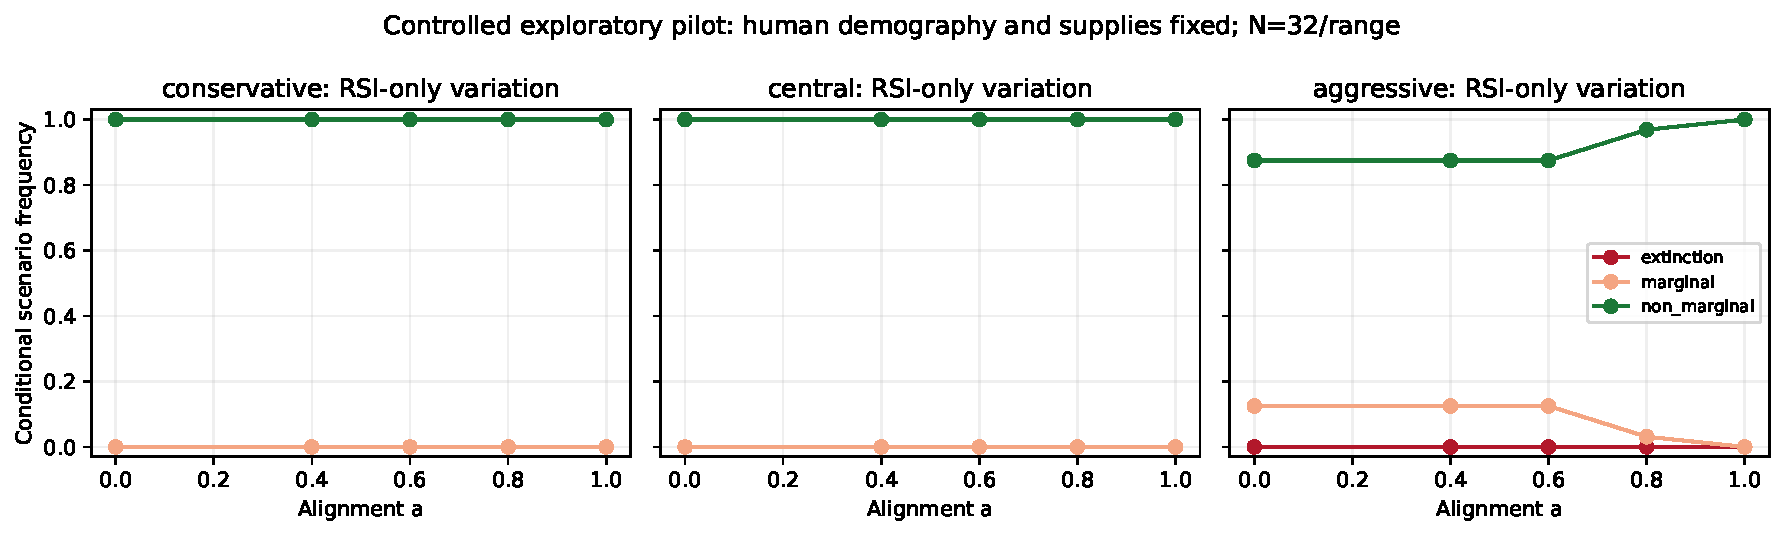
\includegraphics[width=\textwidth]{p0_controlled_rsi.pdf}
\caption{RSI-only exploratory comparison with human, resource and initial conditions fixed.
No population or resource parameter is changed to obtain a desired outcome.}
\end{figure}

Since $\dot H\ge-\delta_HH$, $H(t)\ge H_0e^{-\delta_Ht}$.
For the fixed pilot its year-100 lower bound is $2.943\times10^9>H_{\rm ext}$,
so extinction is analytically excluded. For the old joint UQ, individual parameters
must be used: the bound excludes extinction for 45/100 conservative and 33/100 central
vectors, not all vectors. No recorded event violates its own lower bound.

Numerical checking compares 26 targeted cases against a tighter adaptive reference.
All 26 adaptive comparisons pass the configured limits. Old RK4 saved trajectories
pass those limits in only 5/26, 8/26 and 23/26 cases at 1, 0.5 and 0.25 year steps;
all 104 solver comparisons agree on outcome class. Output interpolation contributes
to trajectory errors. A further 12 stratified random parameter vectors, paired across
three alignments, produce 36 checks with no failures or class changes. These are not
36 independent parameter draws or a certificate for the entire 4,400-run library.
The interrupted full-library recheck remains incomplete.

\section{Discussion and handoff limitations}
The contribution is integration of a shared allocator, physical hardware constraints,
industrial dependence and a conditional safety certificate, not new KKT or invariance
theory. Historical compatibility, uncertain hardware units, exogenous power, fixed land
partitions, aggregate demographics and completed-decommissioning assumptions limit
interpretation. Earlier rank associations and finite-grid robust sets are exploratory;
no unique measurement priority, causal effect, continuous viability kernel or EVPI
is established. Equality comparisons use a documented $10^{-10}$ numerical tolerance;
threshold-event resolution remains finite.

P0 is handed off as a runnable, selectively verified research prototype. Part V
intervention/timing comparison, source verification, the complete final paper,
Summary Sheet, ENOCH letter and AI-use report remain later tasks. This LaTeX source
has not been compiled in the current environment. Detailed equations, all earlier
figures and proofs are retained in the mathematical specification and archived draft.
\end{document}
